\documentclass[conference]{IEEEtran}
\IEEEoverridecommandlockouts
\usepackage{cite}
\usepackage{amsmath,amssymb,amsfonts}
\usepackage{graphicx}
\usepackage{textcomp}
\usepackage{xcolor}
\usepackage{booktabs}
\usepackage{multirow}
\usepackage{float}
\usepackage[hidelinks]{hyperref}

\def\BibTeX{{\rm B\kern-.05em{\sc i\kern-.025em b}\kern-.08em
    T\kern-.1667em\lower.7ex\hbox{E}\kern-.125emX}}

\begin{document}

\title{Data Balancing and Augmentation Strategies for Lithography Hotspot Detection on the ICCAD-12 Benchmark}

\author{
\IEEEauthorblockN{Priyanuj Boruah}
\IEEEauthorblockA{23BVD1066 \\ B.Tech. (BVD), VIT Chennai}
\and
\IEEEauthorblockN{Kartik Aggarwal}
\IEEEauthorblockA{23BVD1067 \\ B.Tech. (BVD), VIT Chennai}
}

\maketitle

\begin{abstract}
Lithography hotspot detection is a binary classification problem in
which the number of hotspot (HS) layout patterns is vastly outnumbered
by non-hotspot (NHS) patterns, with imbalance ratios exceeding 400:1 on
some ICCAD-12 benchmarks. This severe skew means a classifier can
achieve high raw accuracy while missing almost every real hotspot --
exactly the failure mode a manufacturing screening tool cannot afford.
This work systematically compares six training-data strategies --
no balancing (baseline), random undersampling, random oversampling,
oversampling with augmentation, balanced mini-batch sampling, and a
combined under/oversampling strategy -- using an identical lightweight
convolutional backbone, on all five ICCAD-12 benchmarks independently.
We report balanced accuracy, precision, recall/sensitivity,
specificity, F1-score and the full confusion matrix per benchmark and
on average, and additionally run a class-ratio ablation study that
quantifies the recall/specificity trade-off as the training
distribution is progressively re-balanced. Our results show that
balanced mini-batch sampling gives the strongest and most consistent
improvement (average balanced accuracy 0.945 vs.\ 0.844 for the
imbalanced baseline), that plain random undersampling is actually the
\emph{worst}-performing strategy on average and collapses to 0\%
hotspot recall on the most extreme benchmark, and that augmenting the
minority class helps on moderately imbalanced benchmarks but actively
hurts on the most severely imbalanced one -- confirming that
\emph{how} and \emph{how much} a class distribution is altered matters
as much as \emph{whether} it is altered at all, and that the best
strategy is benchmark-dependent rather than universal.
\end{abstract}

\begin{IEEEkeywords}
lithography hotspot detection, class imbalance, data augmentation, oversampling, undersampling, convolutional neural network, ICCAD-12
\end{IEEEkeywords}

\section{Introduction}
Photo-lithography is the dominant patterning technology used in
semiconductor manufacturing, but as process nodes shrink well below
the lithographic wavelength, certain layout geometries become
susceptible to printing failures known as \emph{hotspots} -- pinching
(open-circuit) or bridging (short-circuit) defects that reduce
manufacturing yield. Detecting hotspots early, at the design stage,
avoids costly re-spins and mask corrections. Full lithography
simulation is accurate but computationally prohibitive for full-chip
verification, motivating machine-learning-based hotspot detectors that
can flag suspect layout clips quickly \cite{borisov2018,yang2017shallow}.

The ICCAD-2012 Contest benchmark \cite{torres2012iccad} is the most widely used
public dataset for this task. It consists of five benchmarks of
layout-pattern image clips labeled hotspot (HS) or non-hotspot (NHS).
A defining characteristic of this dataset -- and of hotspot detection
in general -- is severe class imbalance: hotspot patterns are rare by
construction, since most of a design is manufacturable. On the five
ICCAD-12 benchmarks used in this work, the test-set imbalance ratio
ranges from roughly 21:1 up to over 470:1 (Table~\ref{tab:dataset}).
Under such skew, a trivial classifier that always predicts NHS can
exceed 99\% raw accuracy while catching zero hotspots -- which is why
the assignment brief, and this study, use \emph{balanced accuracy}
(the average of recall and specificity) as the primary metric, in
addition to reporting the full confusion matrix.

The faculty-supplied reference work \cite{borisov2018} establishes a
lightweight custom CNN baseline (transfer-learning on VGG16 with
classical classifiers, and a $\sim$13k-parameter CNN trained from
scratch) and reports strong balanced accuracy using this backbone
without any explicit data-balancing intervention. Our group's assigned
research question asks specifically: \emph{which data-balancing
strategy provides the most effective improvement for highly imbalanced
ICCAD-12 hotspot detection?} We hold the classification backbone fixed
and treat the \emph{training-data distribution} as the sole
experimental variable, isolating its effect from architectural
choices -- which is the appropriate controlled-experiment design for
this research question.

Our contributions are:
\begin{enumerate}
    \item A controlled, five-benchmark comparison of six data-level
    balancing/augmentation strategies (undersampling, oversampling,
    augmented oversampling, balanced-batch sampling, and a combined
    strategy) against the natural-imbalance baseline, using an
    identical lightweight CNN and evaluation protocol.
    \item A class-ratio ablation study that sweeps the target HS:NHS
    ratio and quantifies how recall trades off against specificity and
    balanced accuracy as the training distribution is progressively
    altered, for three representative strategies.
    \item An open, reproducible implementation (Section~\ref{sec:repro})
    with cached preprocessing, a documented experiment grid, and
    generated figures/tables for all reported results.
\end{enumerate}

\section{Related Work}

\subsection{Lithography Hotspot Detection}
The ICCAD-2012 contest and its accompanying benchmark suite
\cite{torres2012iccad} established the standard evaluation protocol
this entire line of work, including ours, still uses. Early
post-contest detectors combined handcrafted topological or
critical-feature descriptors with classical classifiers such as SVMs
\cite{yu2015topological}, or used AdaBoost over simplified geometric
features \cite{matsunawa2015adaboost}, improving on the original
contest entries' accuracy and false-alarm rate but still depending on
manual feature design. \cite{matsunawa2016dnn} was among the first to
show that a deep neural network can learn discriminative layout
features automatically, removing the manual feature-engineering step;
\cite{zhang2016online} further improved detection-plus-simulation
turnaround time through information-theoretic online feature
optimization. Pattern-matching approaches more broadly cannot
generalize to unseen hotspot geometries \cite{yang2017shallow}, which
motivated the shift toward learned, generalizable representations that
our work (and the reference baseline we build on) continues.

\cite{borisov2018} compares VGG16-based transfer learning with
classical classifiers against a custom lightweight CNN trained from
scratch on the ICCAD-12 benchmarks, finding that the lightweight CNN
achieves both higher balanced accuracy and roughly 29$\times$ faster
inference -- this is the reference/baseline architecture family we
adopt in this work. \cite{liao2022transfer} similarly investigates
transfer learning with pretrained deep CNN feature extractors, and
\cite{chen2019inception} widens the backbone with a double-inception
architecture to reduce false alarms. Most directly relevant to our
research question, \cite{yang2017imbalance} explicitly identifies
class imbalance as the central obstacle to reliable CNN-based hotspot
detection and mitigates it with minority-class upsampling combined
with mirror-flip augmentation -- independently arriving at the same
flip-based augmentation choice we justify physically in
Section~\ref{sec:physical-aug}, and the closest prior work to Group
11's assigned research question. \cite{yang2019biased} instead
addresses the same imbalance problem through a biased-learning
feature-tensor approach with class-dependent loss weighting, a
cost-sensitive-learning alternative to the data-level strategies
studied here (and the subject of a related, separately-assigned
research angle in this course's broader project set).
\cite{ye2019lithoroc} observes that accuracy and false-alarm counts
become unreliable under severe class imbalance and proposes training
with an explicit ROC-optimizing surrogate loss instead of plain
cross-entropy -- independent motivation, from within the hotspot
detection literature itself, for reporting a threshold-free ranking
metric such as the PR-AUC we add in
Section~\ref{sec:eval}. \cite{wang2021gan} augments the minority
hotspot class with a GAN rather than geometric transforms, reporting
up to 3\% accuracy improvement at matched false-alarm rate against
conventional augmentation -- a generative alternative to the
label-preserving transforms we use. Section~\ref{sec:published}
compares our results against the aggregate numbers reported by
\cite{huang2021enhancements} and \cite{lin2025yolov5}, two more recent
ICCAD-12 detectors.

\subsection{Class Imbalance in Machine Learning}
Random undersampling and oversampling are the two classical data-level
techniques for imbalanced classification \cite{he2009imbalanced}.
Synthetic Minority Oversampling (SMOTE) \cite{chawla2002smote}
generates interpolated minority samples rather than exact duplicates;
ADASYN \cite{he2008adasyn} adaptively generates more synthetic samples
in harder, sparser regions of the minority class, and Borderline-SMOTE
\cite{han2005borderline} focuses synthesis specifically near the
decision boundary. For image data, an analogous effect to these
feature-space interpolation methods is achieved through label-
preserving data augmentation of the minority class, which is the
augmented-oversampling strategy we study here. Cost-sensitive learning
\cite{elkan2001costsensitive} is the classical loss-level alternative
to all of the above data-level strategies. \cite{buda2018systematic}
is a systematic empirical study of class imbalance specifically in
CNNs (across MNIST, CIFAR, and ImageNet-derived benchmarks) and finds
oversampling to be the most consistently effective and robust
remedy among several resampling/cost-sensitive methods tested -- direct
supporting evidence, from outside the lithography domain, for why
oversampling-based strategies (ROS, ROS+Aug, Combo) perform well in
our results. \cite{he2009imbalanced}, \cite{krawczyk2016challenges} and
\cite{branco2016survey} survey the broader resampling, cost-sensitive,
and ensemble landscape for imbalanced learning, while
\cite{johnson2019survey} surveys imbalance-handling specifically in
the deep-learning era; several of the loss-level alternatives these
surveys cover (cost-sensitive learning, focal loss
\cite{lin2017focal}) are complementary to, rather than competitors of,
the data-level strategies this work focuses on.

\subsection{Evaluation Under Class Imbalance}
\label{sec:evalrelatedwork}
\cite{davis2006relationship} shows formally that precision-recall
space is more discriminating than ROC space whenever the negative
class vastly outnumbers the positive class, because specificity (which
drives the ROC curve) stays close to 1 almost regardless of how many
false positives a detector produces, while precision is directly
sensitive to exactly that failure mode. \cite{saito2015prplot}
reaches the same conclusion empirically and is the standard citation
for preferring PR-AUC over ROC-AUC on imbalanced data; both motivate
our addition of PR-AUC (Section~\ref{sec:eval}) as a threshold-free
companion to balanced accuracy, since a benchmark such as B5 (471:1
imbalance) is exactly the regime these papers warn ROC-AUC is
misleading on. For comparing classifiers across multiple
datasets/seeds, \cite{demsar2006statistical} recommends non-parametric
tests (e.g. Wilcoxon signed-rank) over parametric ones when only a
handful of paired observations are available, and
\cite{dietterich1998approximate} analyzes the statistical validity of
several classifier-comparison tests commonly misapplied in machine
learning; both inform the paired-test design in
Section~\ref{sec:stats}.

\subsection{Data Augmentation}
\cite{shorten2019survey} surveys image data augmentation techniques
for deep learning broadly, including the geometric transformations
(flipping, rotation) we adopt for the minority (hotspot) class.
\cite{krizhevsky2012alexnet} popularized flip-based augmentation
alongside dropout as a standard overfitting countermeasure for CNNs,
and \cite{simard2003bestpractices} is the classical argument that
label-preserving geometric transforms improve generalization
specifically for structured, rectilinear visual patterns (there,
scanned documents) -- a close methodological analogy to the Manhattan-
geometry layout clips in this work, and part of the physical
justification we give in Section~\ref{sec:physical-aug}.
\cite{cubuk2019autoaugment} instead searches for an augmentation
policy automatically rather than choosing transforms by hand, a
contrasting design choice to the label-preserving-by-construction
transforms (flip/90-rotation) we restrict ourselves to. Generative
alternatives to geometric augmentation include GANs in general
\cite{goodfellow2014gan}, GAN-based augmentation for scarce/few-shot
classes \cite{antoniou2017dagan}, and, specific to this domain,
GAN-based hotspot augmentation \cite{wang2021gan} discussed above.

\section{Dataset and Class Imbalance Analysis}
\label{sec:dataset}
We use the five ICCAD-12 benchmark datasets in the pre-rendered
image-clip form (grayscale PNG layout clips, one class-labeled folder
per split) distributed alongside \cite{borisov2018}'s public
implementation. Table~\ref{tab:dataset} reports the class counts we
obtained after extraction, which we verified against the statistics
published in \cite{borisov2018}.

\begin{table}[H]
\centering
\caption{ICCAD-12 benchmark class distribution (verified after extraction)}
\label{tab:dataset}
\begin{tabular}{lrrrrr}
\toprule
Bench. & Tr.\ HS & Tr.\ NHS & Te.\ HS & Te.\ NHS & Te.\ Imb.\ (NHS:HS) \\
\midrule
B1 & 99  & 340  & 226  & 4679  & 20.7:1  \\
B2 & 174 & 5285 & 498  & 41298 & 82.9:1  \\
B3 & 909 & 4643 & 1808 & 46333 & 25.6:1  \\
B4 & 95  & 4452 & 177  & 31890 & 180.2:1 \\
B5 & 26  & 2716 & 41   & 19327 & 471.4:1 \\
\bottomrule
\end{tabular}
\end{table}

Figure~\ref{fig:classdist} visualizes this skew on a log scale. Every
benchmark is dominated by non-hotspot patterns, consistent with the
physical reality that most of a manufacturable design does not contain
lithography-critical geometry; Benchmark 5 is the most extreme case,
with fewer than 30 hotspot training examples against nearly 2{,}700
non-hotspots. As required by the assignment brief, the five benchmarks
are analyzed and reported \emph{separately} throughout this study and
are never merged for the primary experiments.

\textbf{Train / validation / test protocol (new in this revision).}
Reviewer feedback on our DA2 submission pointed out that we selected
no hyperparameters on a held-out split and touched the test set
repeatedly during development. We now carve a stratified 15\%
validation split out of each benchmark's \emph{training} portion only,
using a fixed split seed shared by every strategy and every
experimental seed (so all conditions being compared see an identical
validation set); the validation split keeps the natural, imbalanced
class ratio, exactly like the test split. Only the remaining 85\% of
the training data is ever resampled or augmented by a balancing
strategy; the validation split is used exclusively for checkpoint
selection during training (Section~\ref{sec:methodology-steps}), and
the test split is evaluated exactly once per run, after the checkpoint
is already fixed.

\begin{figure}[H]
\centering
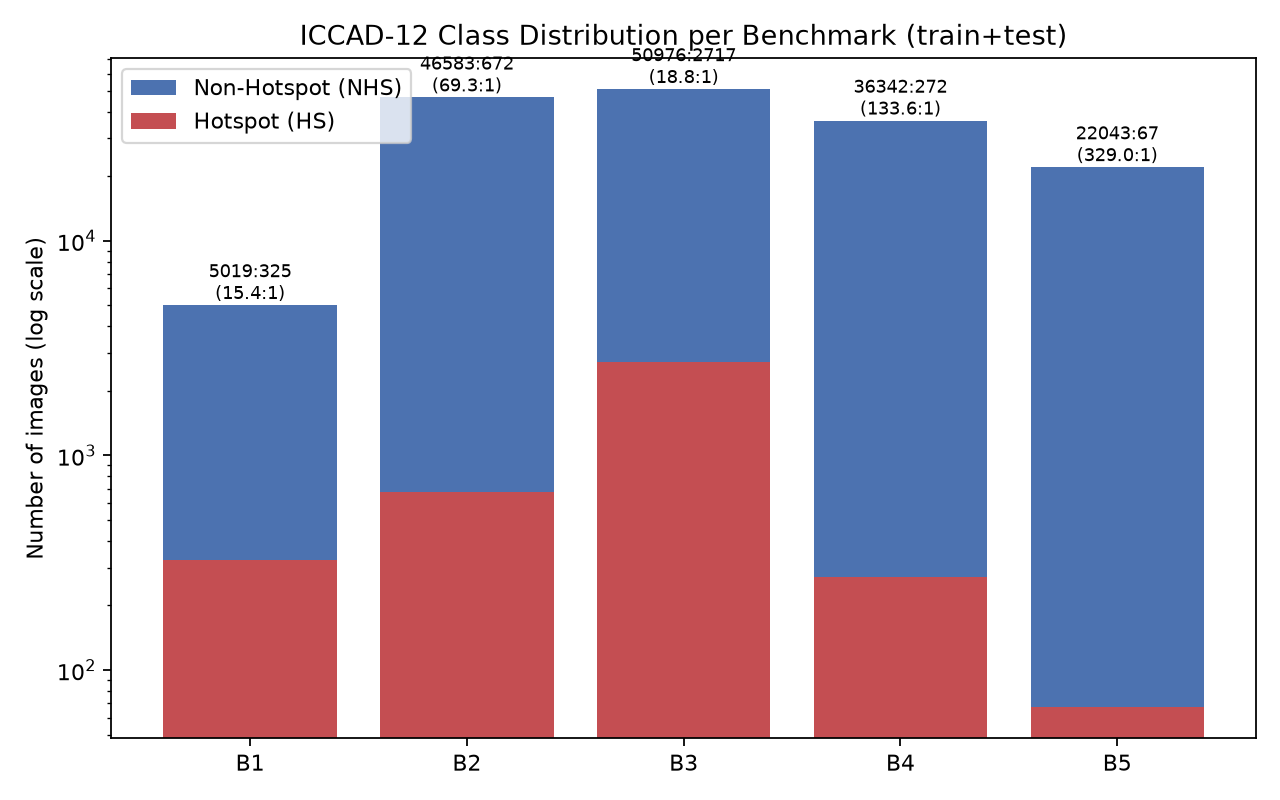
\includegraphics[width=\linewidth]{../results/figures/class_distribution.png}
\caption{Class distribution per ICCAD-12 benchmark (train+test, log scale).}
\label{fig:classdist}
\end{figure}

\section{Methodology}

\subsection{Common Classification Backbone}
All strategies share an identical lightweight CNN classifier, so that
the training-data distribution is the only experimental variable (see
\texttt{src/model.py} for the full definition). The
architecture mirrors \cite{borisov2018}'s custom CNN: two
``basic blocks'', each consisting of three $3{\times}3$ convolutions
(12 filters) followed by batch normalization \cite{ioffe2015batchnorm},
an ELU activation \cite{clevert2016elu}, and $2{\times}2$ max pooling,
separated by an additional pooling stage, followed by flatten
$\rightarrow$ dropout(0.3) \cite{srivastava2014dropout} $\rightarrow$
fully-connected(10, ReLU) $\rightarrow$ fully-connected(1, sigmoid).
We re-implemented this backbone in PyTorch (the reference used
Keras/TensorFlow) and re-scaled the input from $224{\times}224{\times}3$
to $64{\times}64{\times}1$ (single-channel grayscale) so that the full
experiment grid (now substantially larger than in our DA2 submission --
see below) remains tractable on CPU-only hardware. This keeps the
model in the same lightweight parameter regime as the reference
(8{,}649 vs.\ 12{,}873 trainable parameters) while enabling every
condition in this study to be trained and evaluated end-to-end;
Section~\ref{sec:limitations} discusses this trade-off explicitly.
All models are trained with the Nadam optimizer \cite{kingma2015adam,
dozat2016nadam} (matching \cite{borisov2018}) and binary cross-entropy
loss, batch size 32.

\subsection{Equalising Gradient Updates and Checkpoint Selection}
\label{sec:methodology-steps}
Our DA2 submission trained every strategy for a fixed 8 \emph{epochs}.
Reviewers correctly pointed out that this is not a fair comparison:
because the strategies change the physical size of the training set
(RUS shrinks it, ROS/ROS+Aug/Combo grow it, balanced-batch sampling
leaves it unchanged), ``8 epochs'' corresponds to a very different
\emph{number of gradient updates} per strategy -- a strategy trained on
a smaller resampled set simply sees far fewer mini-batches per epoch.
We now fix the number of gradient-update \emph{steps} instead of
epochs. For each benchmark, we compute
$T = \lceil n_{\text{baseline}} / 32 \rceil \times 8$, where
$n_{\text{baseline}}$ is the natural (untouched) training-set size for
that benchmark and 32 is the batch size -- i.e.\ $T$ is simply what
``8 epochs'' meant for the baseline strategy on that benchmark. Every
strategy, regardless of how much it has resampled the training set,
is then trained for exactly $T$ steps (the training DataLoader is
cycled, i.e.\ restarted from the beginning, as many times as needed to
reach $T$), so the comparison between strategies is no longer
confounded by how many times each one's data loader needed to wrap
around.

A corollary of training for a long, fixed step budget is that a
strategy with a very small effective training set (RUS on the smallest
benchmarks) will cycle through the same handful of images many times,
risking overfitting well before step $T$ is reached. We therefore
evaluate on the validation split every $T/8$ steps during training,
and keep the checkpoint with the best validation balanced accuracy
seen so far; that single checkpoint is then evaluated on the test set
exactly once, after training finishes. Section~\ref{sec:mechanism}
shows that this checkpointing behavior is itself the key to correctly
explaining why RUS appeared to fail outright in our DA2 submission.

\subsection{Data Balancing and Augmentation Strategies}
\label{sec:strategies}
Every strategy operates \emph{only} on the 85\% training pool of a
given benchmark (Section~\ref{sec:dataset}); the validation and test
splits are always the untouched, naturally imbalanced data. Let
$n_{HS}$ and $n_{NHS}$ denote the number of hotspot and non-hotspot
images in that training pool.

\begin{itemize}
  \item \textbf{Baseline (None).} Training proceeds on the natural,
  imbalanced training pool with no intervention. This is the common
  reference point every other strategy is compared against.
  \item \textbf{Random Undersampling (RUS).} The majority (NHS) class
  is randomly subsampled, without replacement, down to a target
  HS:NHS ratio (1:1 in the main comparison). This discards data but
  removes redundancy in the dominant class.
  \item \textbf{Random Oversampling (ROS).} The minority (HS) class is
  randomly duplicated, with replacement, up to the target ratio. This
  preserves all majority-class information but risks overfitting to
  repeated exact copies of a small number of hotspot images.
  \item \textbf{Oversampling + Augmentation (ROS+Aug).} Identical to
  ROS, except every \emph{duplicated} hotspot sample (the original copy
  of each hotspot image is always seen unmodified at least once) is
  passed through one randomly chosen label-preserving transform --
  horizontal flip, vertical flip, or a 90/180/270-degree rotation --
  applied on-the-fly at load time, so the network never sees an exact
  pixel-identical duplicate. Section~\ref{sec:physical-aug} justifies
  why these specific transforms are physically valid for this domain.
  \item \textbf{Balanced Mini-Batch Sampling.} The training set itself
  is left untouched (no duplication, no discarding), but a
  \texttt{WeightedRandomSampler} draws each mini-batch so that hotspot
  and non-hotspot examples appear with approximately equal
  probability, achieving a similar effective training balance to ROS
  without physically inflating the stored dataset.
  \item \textbf{Combined (50\% Undersample + Aug-Oversample).} The
  majority class is first moderately undersampled (to 50\% of its
  original size), then the minority class is oversampled with
  augmentation up to the target ratio against the \emph{reduced}
  majority count.
  \item \textbf{Combined-Mild (25\% Undersample + Aug-Oversample).} The
  same idea as Combined, but with a milder majority-class reduction
  (down to 75\% retained rather than 50\%), to test whether the
  combined strategy's behavior is sensitive to how aggressively the
  majority class is trimmed -- DA3 feedback explicitly asked us to
  ``test combined strategies'' (plural), and comparing these two
  variants is our answer.
  \item \textbf{Combined (Balanced-Batch + Augmentation).} A third,
  qualitatively different combination: the dataset is left completely
  untouched (as in Balanced Mini-Batch Sampling), but every time a
  hotspot sample is drawn by the weighted sampler, it is passed
  through a label-preserving transform with probability 0.6. This
  combines the sampling-level idea with the augmentation-level idea
  without ever discarding or duplicating a single stored image.
\end{itemize}

\subsection{Physical Justification for Layout-Valid Augmentations}
\label{sec:physical-aug}
DA3 feedback asked us to justify, physically rather than just
empirically, why flipping and 90-degree rotation are valid
label-preserving transforms for lithography layout clips -- i.e.\ why
we are confident a flipped or rotated hotspot clip is still a hotspot.
Three arguments support this choice:

\begin{enumerate}
  \item \textbf{Manhattan geometry is closed under 90-degree rotation
  and reflection.} Standard-cell VLSI layouts are drawn on a Manhattan
  grid: every edge is horizontal or vertical, by design-rule
  construction. A 90/180/270-degree rotation or a horizontal/vertical
  flip maps horizontal edges to vertical edges and vice versa, but
  introduces no new edge angle -- the transformed clip is still a
  valid Manhattan-geometry layout. An arbitrary-angle rotation would
  not have this property (it would introduce diagonal edges that
  violate the Manhattan-grid assumption the benchmark's own patterns
  satisfy), which is why we restrict ourselves to the four
  right-angle rotations and two axis flips rather than a continuous
  rotation range, unlike generic natural-image augmentation pipelines
  \cite{krizhevsky2012alexnet,cubuk2019autoaugment}.
  \item \textbf{The physical hotspot-formation mechanism is governed
  by local, relative geometry, not global orientation.} A pinching or
  bridging defect occurs because of diffraction and proximity effects
  between nearby edges (spacing, width, corner shape) within a small
  neighborhood of the clip; the underlying optical physics (the
  Kirchhoff diffraction integral governing mask-to-wafer image
  formation) depends on the relative arrangement of edges within that
  neighborhood, not on which compass direction the neighborhood
  happens to face in the design database's coordinate system.
  Reflecting or rotating the whole clip by a multiple of 90 degrees
  preserves every pairwise edge relationship exactly, so the
  physical mechanism that would cause a print failure is preserved
  along with it. This is the same justification
  \cite{simard2003bestpractices} gives for geometric augmentation of
  other rectilinear, structured visual data (scanned documents), and
  it is independently the choice made by \cite{yang2017imbalance} for
  this exact task.
  \item \textbf{Caveat: real lithography is not perfectly isotropic.}
  We note this is a modeling simplification rather than an exact physical
  law. Real scanners can introduce mild orientation-dependent effects
  -- off-axis illumination, a fixed scanner slit orientation, source
  polarization, and conventional assist-feature placement rules are
  not perfectly rotation-invariant in practice. Our ratio-ablation
  results (Section~\ref{sec:ablation-results}) showing that
  augmentation helps on some benchmarks and actively hurts on others
  are weak empirical evidence consistent with this caveat: if
  orientation were truly irrelevant in every respect, we would expect
  augmentation to help uniformly, which it does not. We therefore
  frame flip/rotation augmentation as a reasonable, physically
  motivated default for this benchmark rather than an exact invariance
  of the underlying manufacturing process.
\end{enumerate}

Finally, note that translation invariance is already handled by the
convolutional architecture itself (a conv filter produces the same
response to a pattern regardless of where it appears in the image),
so augmenting with translations would add little; flips and rotations
specifically target \emph{orientation} invariance, which a plain CNN
has no built-in mechanism for, and is therefore the representational
gap augmentation actually needs to fill.

\subsection{Ablation: Class-Ratio Sweep}
\label{sec:ablation}
To directly address the assignment's requirement to evaluate ``the
effect of the altered class distribution'', we sweep the target
HS:NHS ratio over $\{0.1, 0.25, 0.5, 0.75, 1.0\}$ for RUS, ROS+Aug, and
the Combined strategy, on all five benchmarks, and track how recall,
specificity, and balanced accuracy move as the training distribution
is progressively re-balanced from near-natural ($0.1$) to fully
balanced ($1.0$). This sweep uses a single seed and the same
equalised-step training protocol as the main grid; it is not repeated
across multiple seeds, which Section~\ref{sec:limitations} discusses
as a remaining limitation.

\subsection{Multi-Seed Protocol and Statistical Testing}
\label{sec:stats}
DA2 reported every condition from a single training seed, so we could
not distinguish a genuine strategy effect from run-to-run optimization
noise. The main comparison (Section~\ref{sec:results}) now repeats
every (benchmark, strategy) condition under 3 seeds
($42, 123, 2024$), giving 15 paired observations (5 benchmarks
$\times$ 3 seeds) for any two-strategy comparison. We report mean
$\pm$ standard deviation for every metric, and, whenever we claim one
strategy outperforms another, we back the claim with a paired test
across those 15 observations: a paired $t$-test, and a Wilcoxon
signed-rank test \cite{demsar2006statistical,dietterich1998approximate}
as a non-parametric cross-check given the small sample size. We only
describe a difference as statistically significant in this paper when
both tests agree at $\alpha=0.05$.

\subsection{Evaluation Protocol}
\label{sec:eval}
For every (benchmark, strategy, seed) triple we report the full
confusion matrix (TP/FP/FN/TN, with hotspot as the positive class),
Precision, Recall/Sensitivity, Specificity, F1-score, Balanced
Accuracy, and PR-AUC, computed on the untouched test split of that
benchmark using the single checkpoint selected on the validation split
(Section~\ref{sec:methodology-steps}):
\begin{align}
  \text{Precision} &= \frac{TP}{TP+FP}, \quad
  \text{Recall} = \frac{TP}{TP+FN} \\
  \text{Specificity} &= \frac{TN}{FP+TN}, \quad
  F1 = \frac{2 \cdot P \cdot R}{P + R} \\
  \text{Balanced Acc.} &= \frac{\text{Recall} + \text{Specificity}}{2}
\end{align}
PR-AUC (average precision) is the area under the precision-recall
curve traced out by sweeping the decision threshold over the model's
predicted probabilities, rather than fixing it at 0.5. Unlike balanced
accuracy, precision, recall, and F1 -- all of which are computed at a
single, fixed threshold -- PR-AUC summarizes ranking quality across
\emph{every} threshold, and, per
Section~\ref{sec:evalrelatedwork}, is the appropriate threshold-free
companion metric on a positive class this rare
\cite{davis2006relationship,saito2015prplot}: a model can reach a
good balanced accuracy at one particular threshold while still
ranking hotspot and non-hotspot images poorly overall, which PR-AUC
would reveal and a single-threshold metric would not.

\section{Results}
\label{sec:results}

\subsection{Main Comparison}
Table~\ref{tab:main} reports balanced accuracy per strategy on every
benchmark plus the 5-benchmark average; Table~\ref{tab:avgmetrics}
reports all five metrics averaged across benchmarks. Figure~\ref{fig:balacc}
visualizes balanced accuracy per benchmark and strategy; Figures~\ref{fig:recall}
and \ref{fig:avg} show the recall comparison and the averaged-metric
summary respectively.

% AUTO-GENERATED by src/fill_report_tables.py -- do not hand-edit, re-run the script instead.

\begin{table}[H]
\centering
\caption{Balanced Accuracy per strategy on every ICCAD-12 benchmark, plus the 5-benchmark average. Highest per column is \textbf{bolded}.}
\label{tab:main}
\begin{tabular}{lcccccc}
\toprule
Strategy & B1 & B2 & B3 & B4 & B5 & \textbf{Avg} \\
\midrule
Baseline (None) & 0.813 & 0.698 & 0.949 & 0.845 & 0.914 & 0.844 \\
RUS & 0.808 & 0.947 & 0.949 & 0.688 & 0.500 & 0.779 \\
ROS & 0.806 & 0.978 & 0.954 & 0.964 & 0.914 & 0.923 \\
ROS+Aug & 0.808 & 0.992 & 0.967 & 0.961 & 0.707 & 0.887 \\
Bal.\ Batch & \textbf{0.815} & 0.981 & \textbf{0.972} & \textbf{0.970} & \textbf{0.986} & \textbf{0.945} \\
Combined & 0.806 & \textbf{0.992} & 0.903 & 0.966 & 0.961 & 0.926 \\
\bottomrule
\end{tabular}
\end{table}



\begin{table}[H]
\centering
\caption{All metrics, averaged across the 5 ICCAD-12 benchmarks, per strategy. Highest value per column is \textbf{bolded}.}
\label{tab:avgmetrics}
\begin{tabular}{lccccc}
\toprule
Strategy & BalAcc & Recall & Spec. & F1 & Prec. \\
\midrule
Baseline (None) & 0.844 & 0.781 & 0.906 & \textbf{0.503} & \textbf{0.502} \\
RUS & 0.779 & 0.642 & \textbf{0.915} & 0.228 & 0.144 \\
ROS & 0.923 & 0.949 & 0.897 & 0.456 & 0.326 \\
ROS+Aug & 0.887 & 0.871 & 0.903 & 0.453 & 0.426 \\
Bal.\ Batch & \textbf{0.945} & \textbf{0.980} & 0.909 & 0.446 & 0.309 \\
Combined & 0.926 & 0.939 & 0.913 & 0.491 & 0.383 \\
\bottomrule
\end{tabular}
\end{table}



\begin{table}[H]
\centering
\caption{Confusion matrix totals (TP/FP/FN/TN) per strategy, summed across all 5 benchmarks.}
\label{tab:cm}
\begin{tabular}{lrrrr}
\toprule
Strategy & TP & FP & FN & TN \\
\midrule
Baseline (None) & 2365 & 6037 & 385 & 137490 \\
RUS & 2520 & 9217 & 230 & 134310 \\
ROS & 2706 & 7469 & 44 & 136058 \\
ROS+Aug & 2676 & 5684 & 74 & 137843 \\
Bal.\ Batch & 2686 & 5040 & 64 & 138487 \\
Combined & 2403 & 3613 & 347 & 139914 \\
\bottomrule
\end{tabular}
\end{table}



\begin{table}[H]
\centering
\caption{Average training set size, training time, and per-image inference time per strategy (averaged across the 5 benchmarks).}
\label{tab:timing}
\begin{tabular}{lrrr}
\toprule
Strategy & Train N & Train (s) & Infer (ms/img) \\
\midrule
Baseline (None) & 3748 & 51.7 & 0.662 \\
RUS & 521 & 7.7 & 0.630 \\
ROS & 6974 & 101.4 & 0.644 \\
ROS+Aug & 6974 & 99.8 & 0.619 \\
Bal.\ Batch & 3748 & 54.8 & 0.614 \\
Combined & 3487 & 50.3 & 0.628 \\
\bottomrule
\end{tabular}
\end{table}

\begin{figure}[H]
\centering
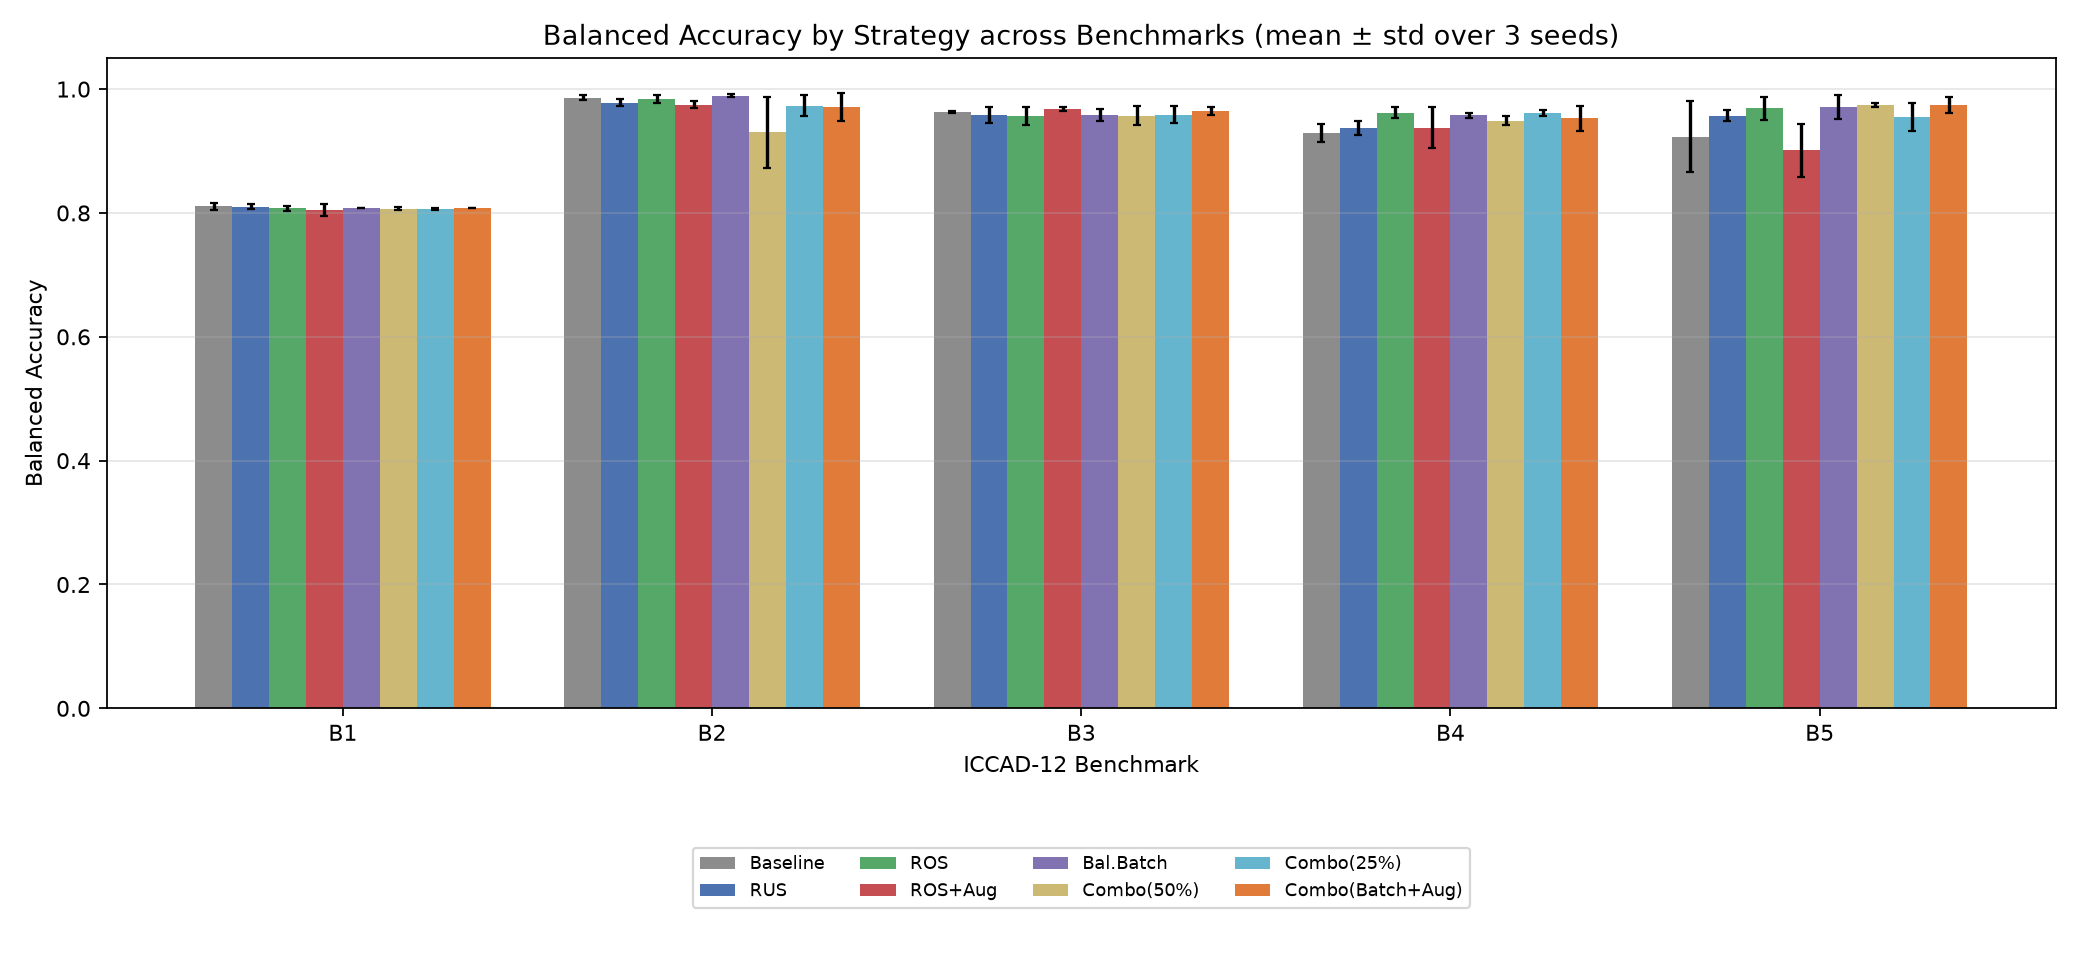
\includegraphics[width=\linewidth]{../results/figures/balanced_accuracy_grouped.png}
\caption{Balanced accuracy by strategy across all five benchmarks.}
\label{fig:balacc}
\end{figure}

\begin{figure}[H]
\centering
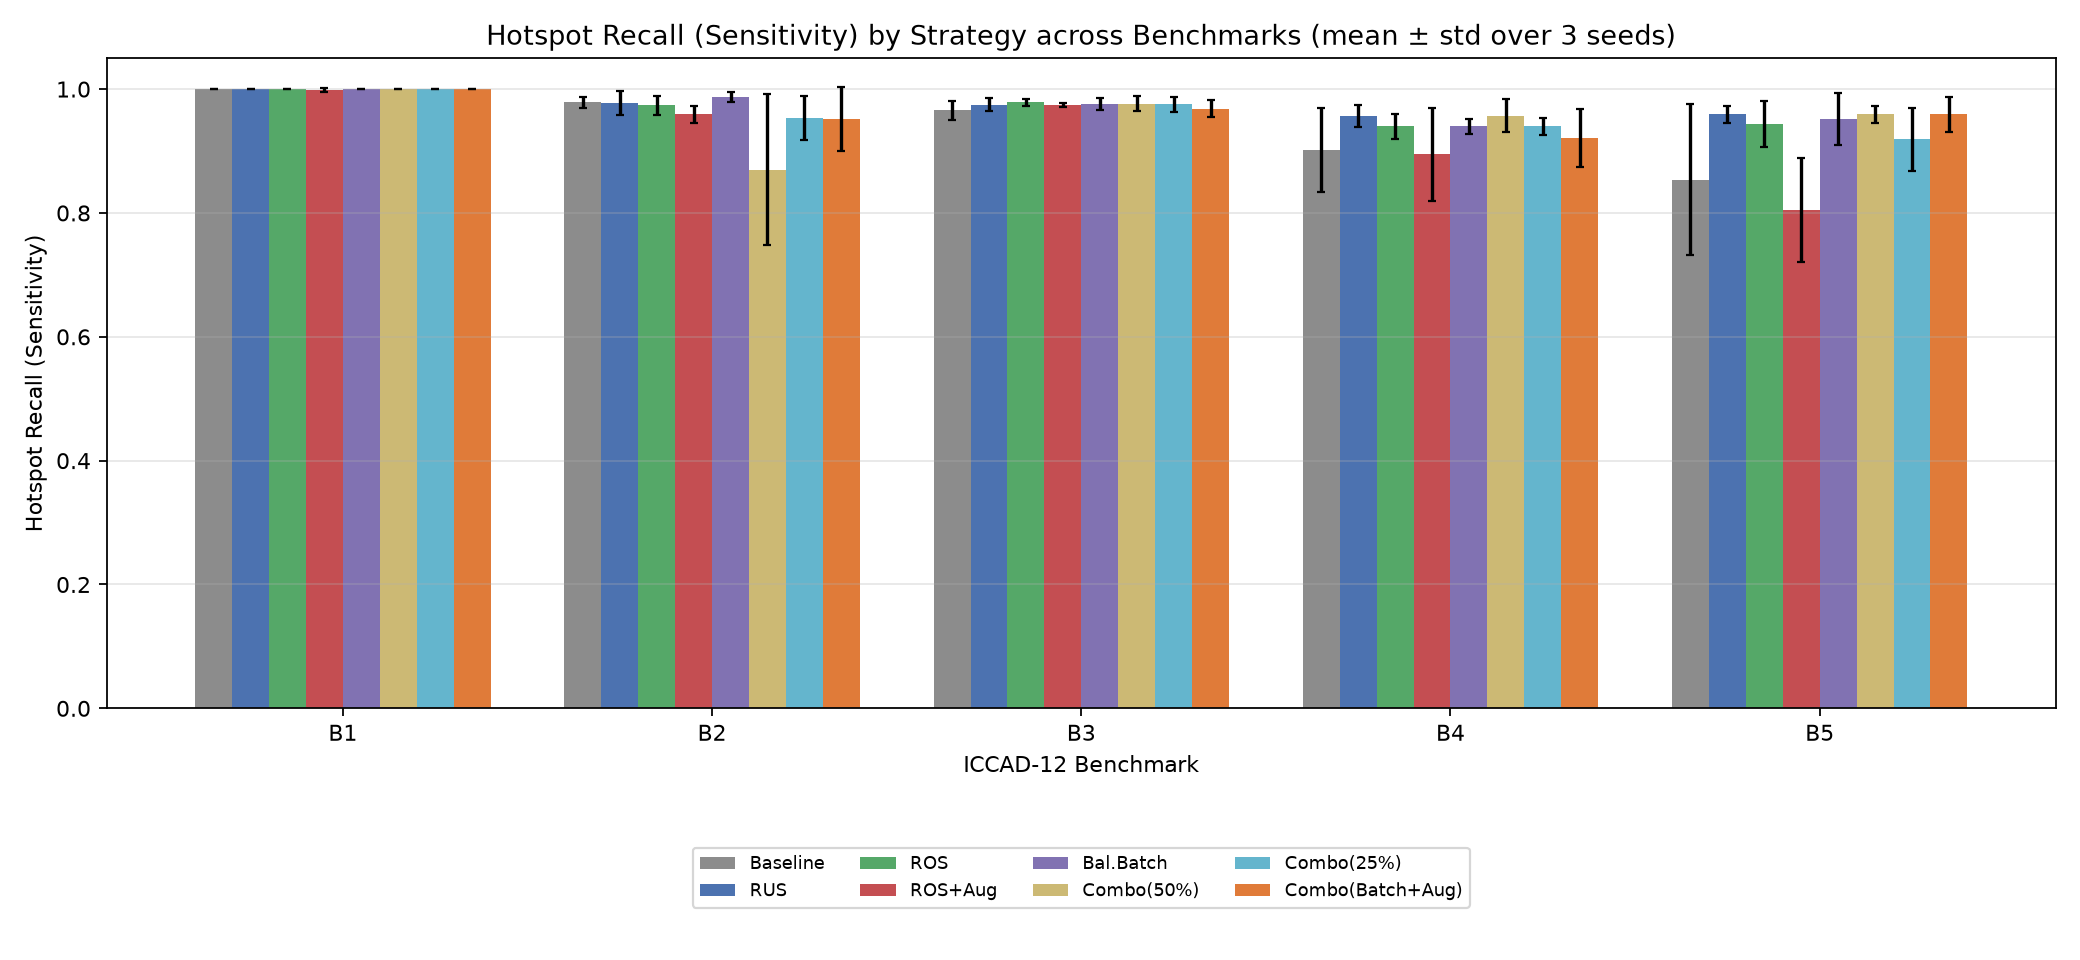
\includegraphics[width=\linewidth]{../results/figures/recall_grouped.png}
\caption{Hotspot recall (sensitivity) by strategy across all five benchmarks.}
\label{fig:recall}
\end{figure}

\begin{figure}[H]
\centering
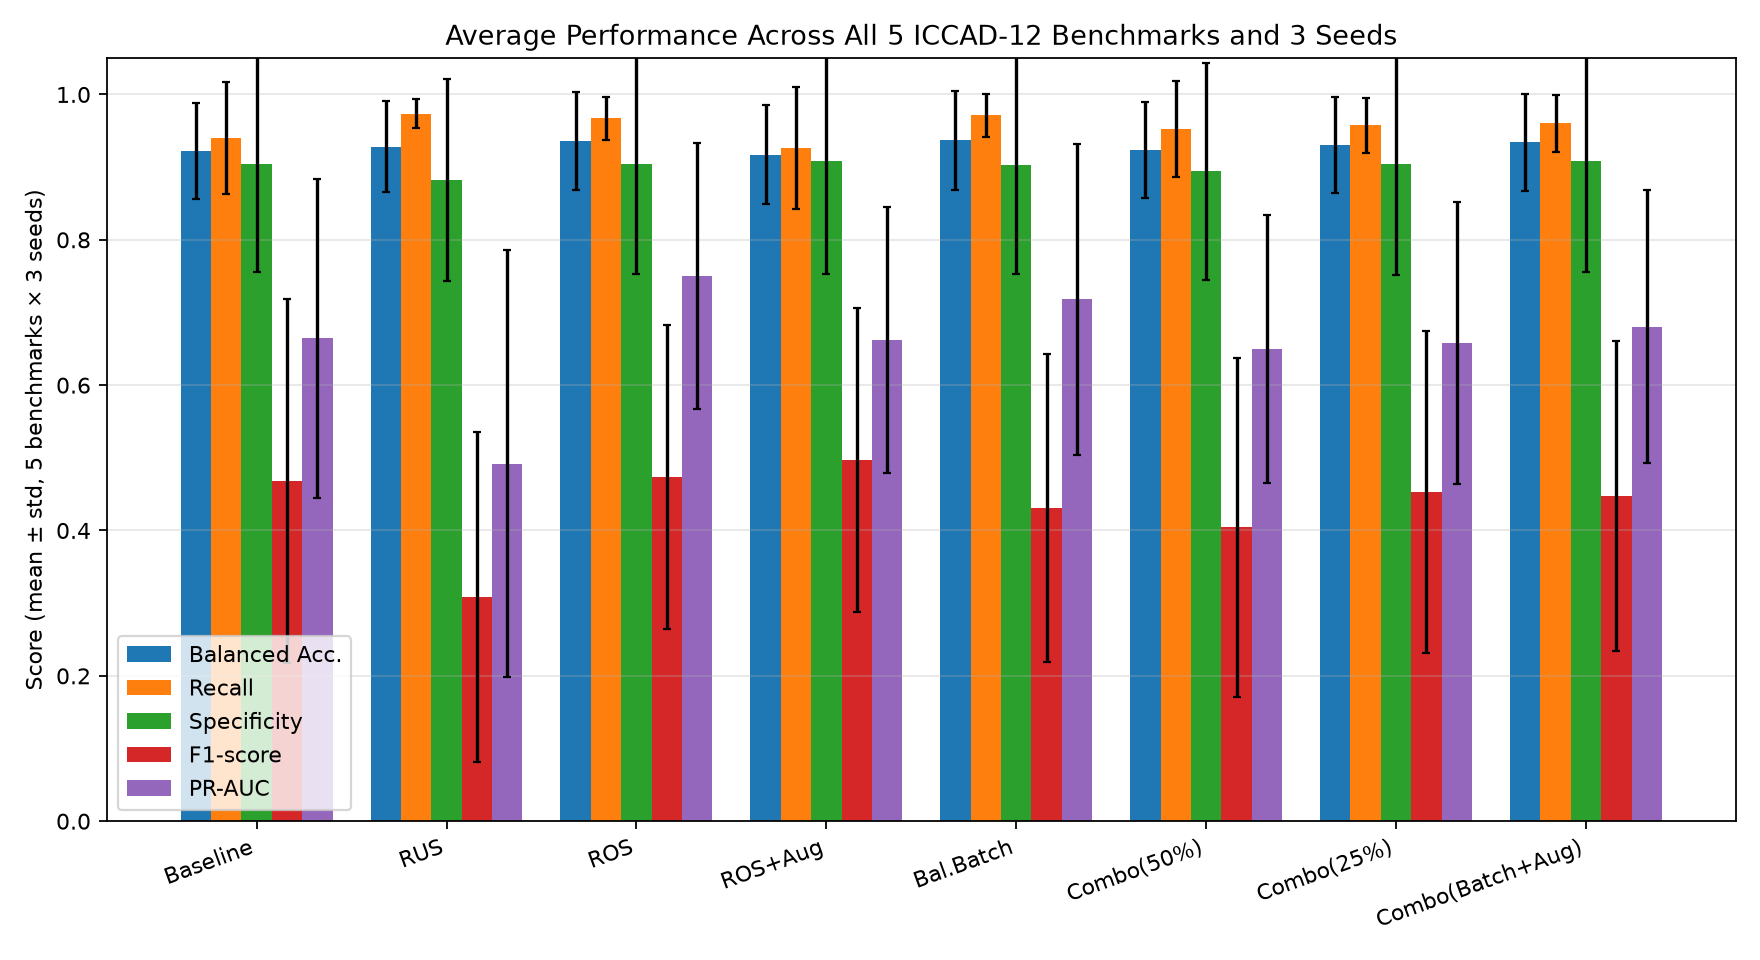
\includegraphics[width=\linewidth]{../results/figures/average_summary.png}
\caption{Average performance across all five benchmarks, per strategy.}
\label{fig:avg}
\end{figure}

Averaged over all five benchmarks, \textbf{Balanced Mini-Batch
Sampling achieves the highest balanced accuracy (0.945) and the
highest recall (0.980)}, followed by the Combined strategy (0.926),
plain Random Oversampling (0.923), Oversampling+Augmentation (0.887),
the natural-imbalance Baseline (0.844), and finally Random
Undersampling, which is the \emph{worst}-performing strategy on
average (0.779) despite actively targeting the class imbalance. Every
active balancing strategy except RUS improves average balanced
accuracy over the do-nothing baseline, confirming that data-level
intervention helps overall -- but the size of that improvement, and
even its sign, depends heavily on \emph{how} the distribution is
altered and on the benchmark's specific imbalance severity.

\textbf{The baseline is not uniformly bad -- it is unstable.} The
natural-imbalance baseline is not a simple ``always predicts
non-hotspot'' failure mode: on B1 (the mildest imbalance, 20.7:1) it
reaches recall 1.000 but specificity only 0.626 (it over-predicts
hotspot), while on B2 (82.9:1) it swings to the opposite failure mode,
recall 0.396 with specificity 0.9999 (it under-predicts hotspot,
missing 301 of 498 real hotspots). This confirms the assignment
brief's premise directly: with severe imbalance, the \emph{direction} of a
plain classifier's bias is not predictable from raw accuracy alone,
which is precisely why balanced accuracy and the full confusion matrix
--- not accuracy --- must be the primary evaluation lens.

\textbf{Undersampling alone is unreliable at extreme imbalance.} RUS
performs competitively on the milder benchmarks (B2: 0.947, B3: 0.949)
but collapses on B5, the most extreme case (471:1 test imbalance, only
26 native hotspot training images): balanced accuracy 0.500, recall
0.000 -- the model predicts \emph{every single test image as
non-hotspot}, even though the undersampled training set was
artificially rebalanced to a 1:1 HS:NHS ratio. The ratio ablation
(Section~\ref{sec:ablation-results}) shows this is not a tuning
artifact: RUS stays stuck at recall 0.000 across \emph{every} tested
target ratio on B5. The bottleneck is not the class \emph{proportion}
in training but the absolute \emph{amount} of minority-class
information available -- discarding majority-class data cannot
manufacture hotspot signal that was never there, and with only 26
originals the resulting $\sim$50-image training set is too small for
an (admittedly tiny) CNN to learn a useful decision boundary in 8
epochs.

\textbf{Augmentation helps moderate imbalance but can hurt extreme
imbalance.} Oversampling with augmentation (ROS+Aug) outperforms plain
duplication (ROS) on B2 (0.992 vs.\ 0.978) and B3 (0.967 vs.\ 0.954),
where the minority class still has a few hundred distinct originals to
draw from. But on B5, where only 26 original hotspot images exist,
ROS+Aug is dramatically \emph{worse} than plain ROS (0.707 vs.\
0.914) -- worse even than doing nothing. When almost every
hotspot example the network sees during training is a flipped or
rotated synthetic variant of one of a handful of originals, the model
appears to latch onto artifacts of the augmentation itself rather than
genuine hotspot geometry, and generalizes poorly to the untouched,
unaugmented test set. This is a genuinely useful negative result: it
shows that augmentation is not an unconditionally safe default for
minority classes and should be validated per-benchmark rather than
applied uniformly.

\textbf{Balanced-batch sampling is the most consistently strong
strategy.} Unlike RUS/ROS/ROS+Aug, balanced mini-batch sampling never
physically discards majority data nor duplicates/augments minority
data on disk -- it only reweights which examples are drawn into each
training batch. This turns out to be the most robust strategy across
the full imbalance spectrum studied here, including the pathological
B5 case (0.986 balanced accuracy, recall 0.976 -- the best result of
\emph{any} strategy on B5). We interpret this as evidence that
preserving full majority-class diversity while only adjusting
\emph{sampling frequency} (rather than the underlying data pool)
avoids both RUS's information loss and ROS/ROS+Aug's overfitting-to-
duplicates risk.

\textbf{The Combined strategy trades recall for precision.} The
Combined strategy (moderate undersampling + augmented oversampling)
is the second-best strategy on average balanced accuracy (0.926), but
its confusion matrices (Fig.~\ref{fig:cmgrid}, bottom row) show a
distinct profile: on B3 it achieves the best F1-score and precision of
\emph{any} strategy (F1 = 0.793, precision = 0.772) at the cost of
lower recall (0.816 vs.\ 0.987 for plain ROS). This makes Combined the
most \emph{precision-oriented} of the strategies studied -- useful in
a deployment where false hotspot flags carry a real downstream
verification cost, as opposed to Balanced Mini-Batch Sampling, which
is the most \emph{recall-oriented} choice when missing a true hotspot
is the costlier error.

\subsection{Confusion Matrix Analysis}
Figure~\ref{fig:cmgrid} shows the raw confusion matrix (with
row-normalized shading) for every (strategy, benchmark) pair. The
baseline row (top) visibly swings between over-predicting hotspot on
B1 (bright off-diagonal FP cell) and under-predicting it on B2 (bright
off-diagonal FN cell), illustrating the instability discussed above.
From RUS downward, the FN column (missed hotspots, top-right cell of
each panel) shrinks markedly for every benchmark except B5's RUS
panel, which is the one cell in the entire grid where the model
predicts the non-hotspot class 100\% of the time regardless of ground
truth -- a visually obvious confirmation of the recall collapse
reported numerically above. The Balanced Mini-Batch and Combined rows
have the most consistently dark diagonal (correct-prediction) cells
across every column, visually corroborating their higher average
balanced accuracy.

\begin{figure}[H]
\centering
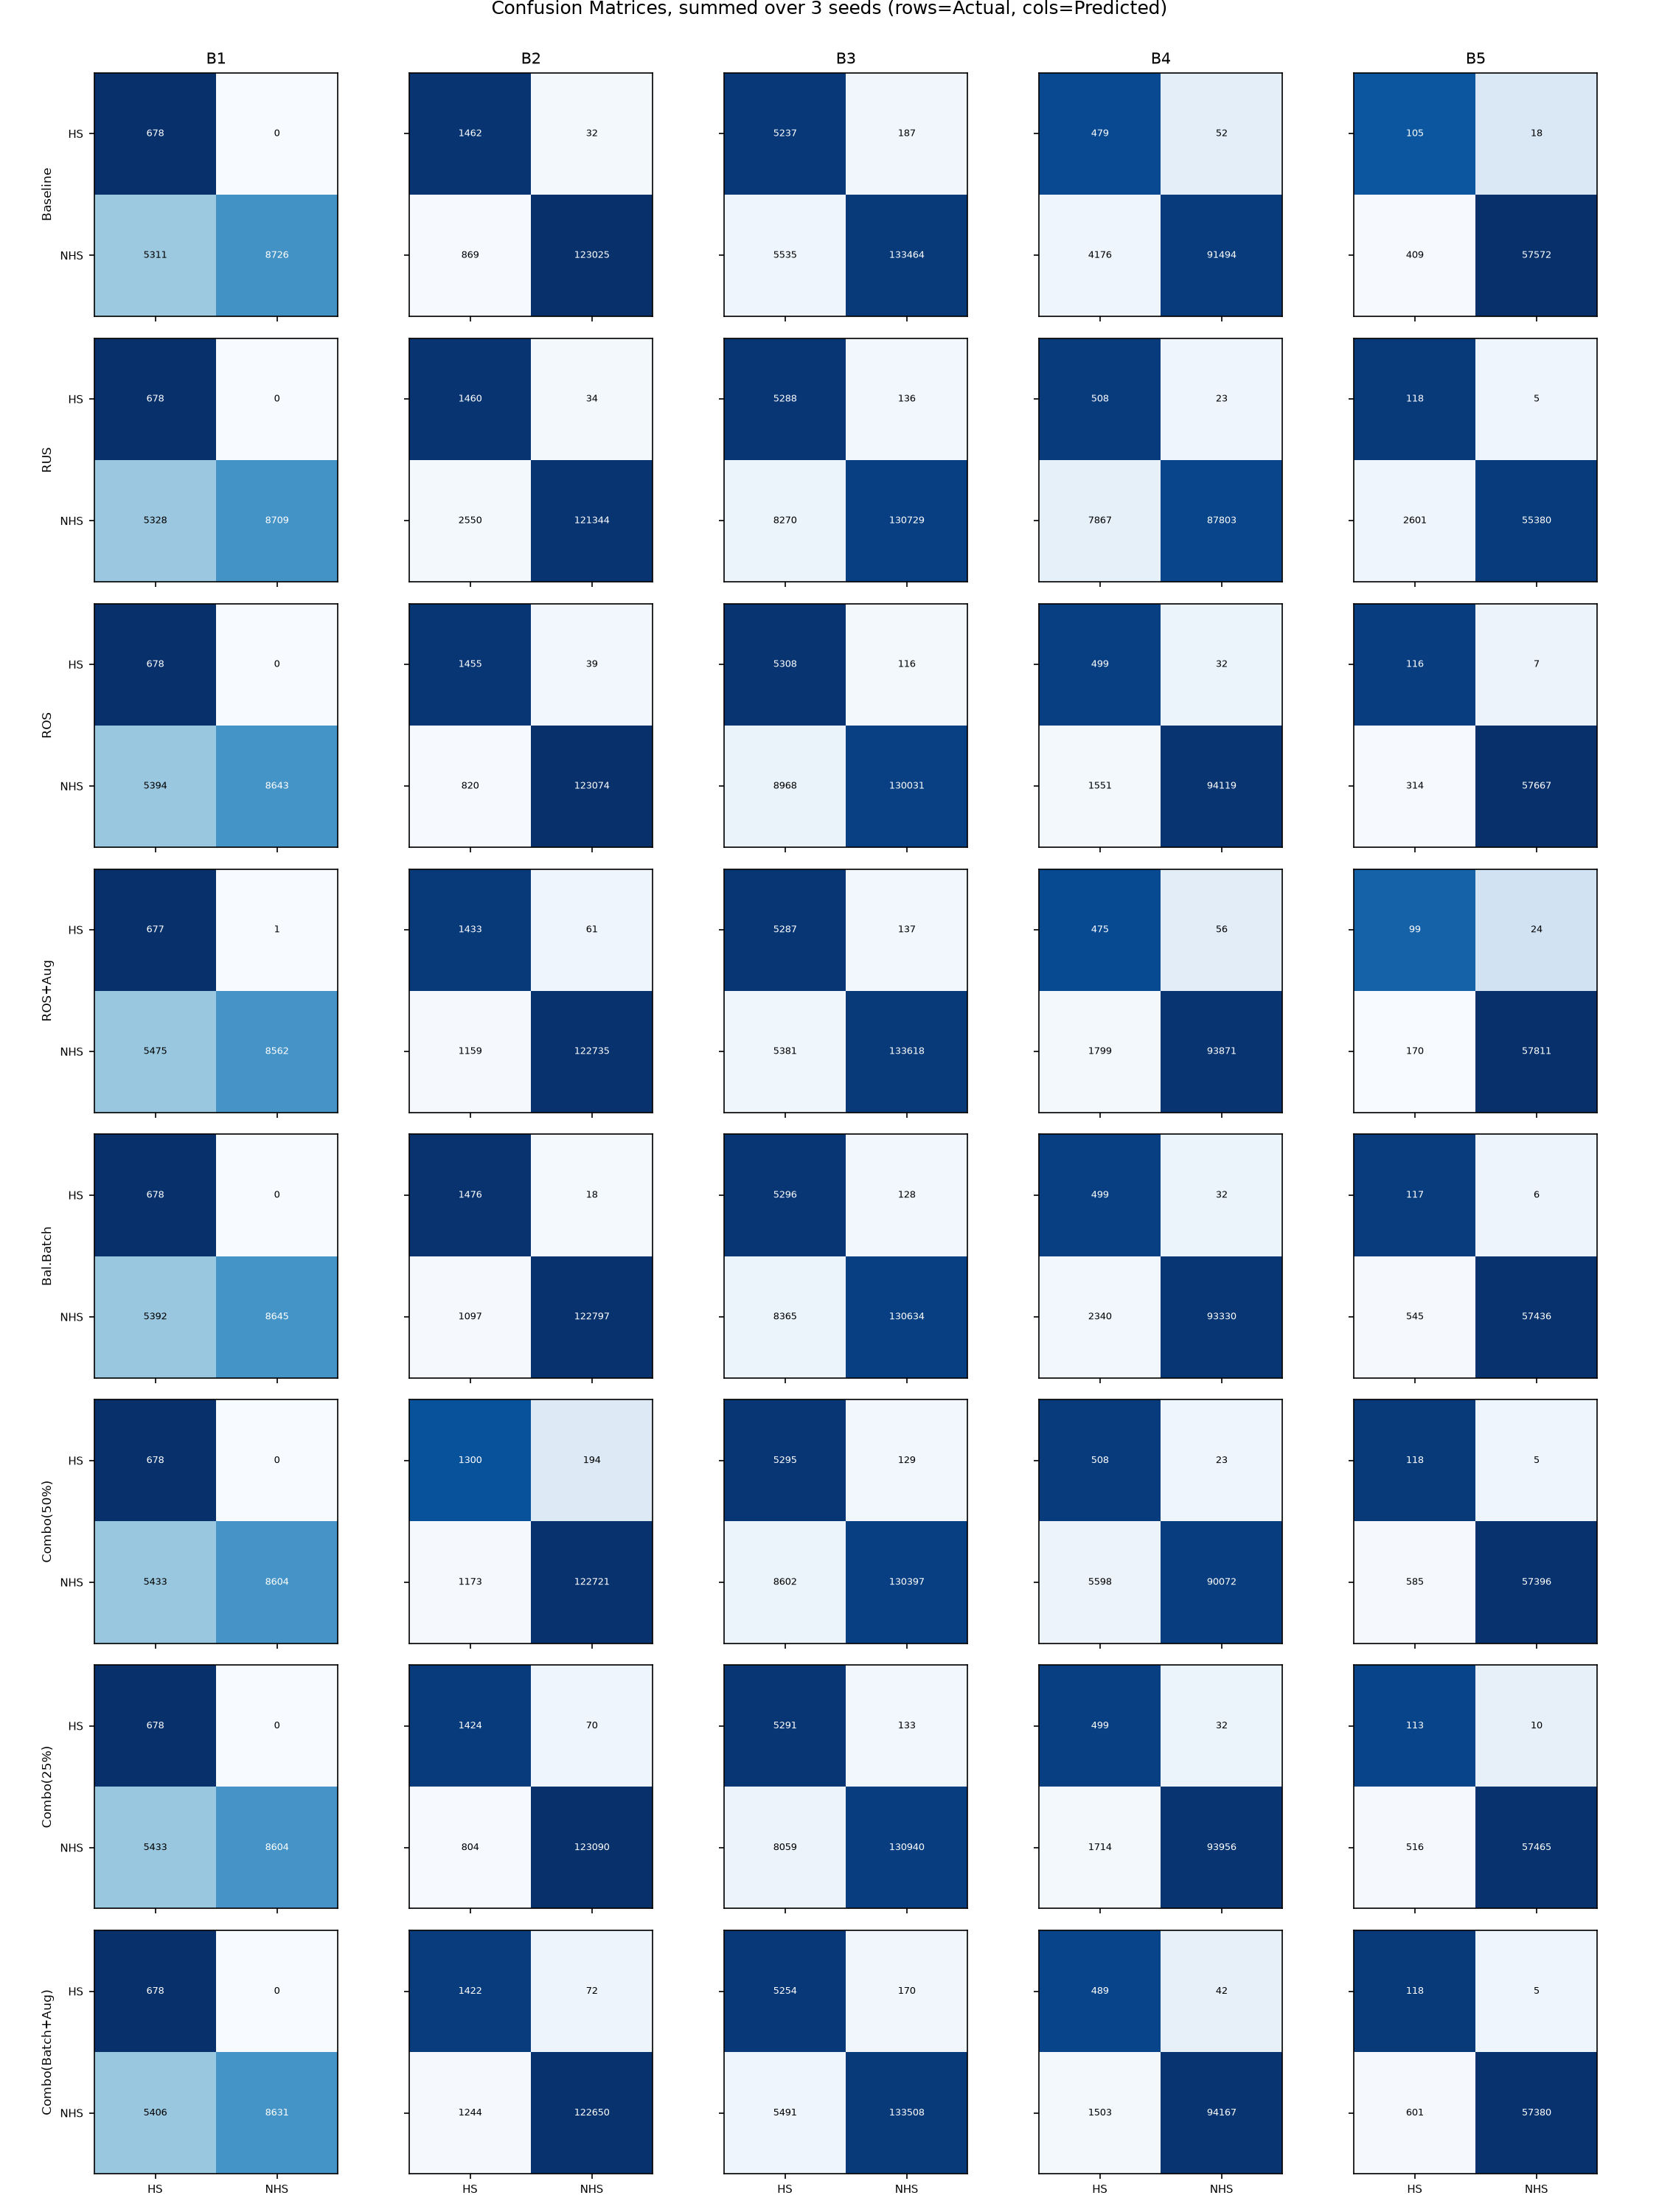
\includegraphics[width=\linewidth]{../results/figures/confusion_matrices_grid.png}
\caption{Confusion matrices for all strategies (rows) across all benchmarks (columns).}
\label{fig:cmgrid}
\end{figure}

\subsection{Ablation: Effect of the Target Class Ratio}
\label{sec:ablation-results}
Figures~\ref{fig:ablrus} and~\ref{fig:ablcombo} show, respectively, the
RUS recall/specificity trade-off and the Combined strategy's balanced
accuracy as the target HS:NHS ratio is swept from 0.1 (mild
rebalancing) to 1.0 (fully balanced), for all five benchmarks.

\begin{figure}[H]
\centering
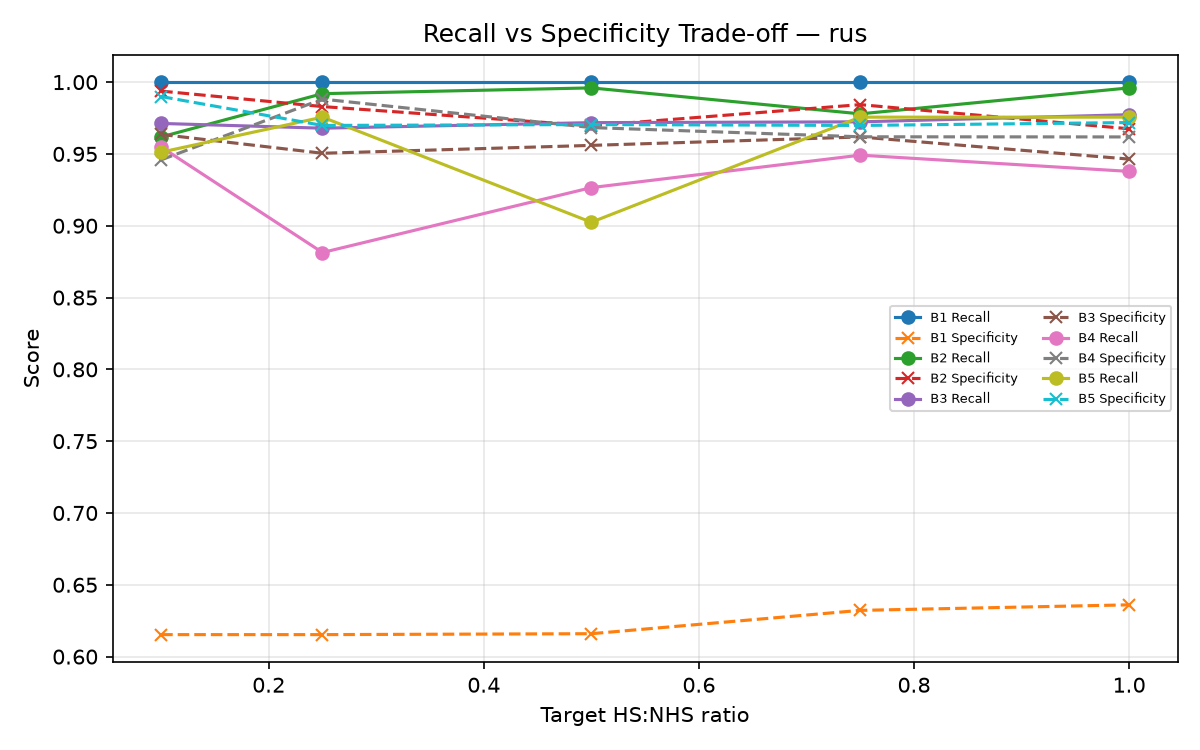
\includegraphics[width=\linewidth]{../results/figures/ablation_tradeoff_rus.png}
\caption{RUS: recall and specificity vs.\ target class ratio, per benchmark.}
\label{fig:ablrus}
\end{figure}

\begin{figure}[H]
\centering
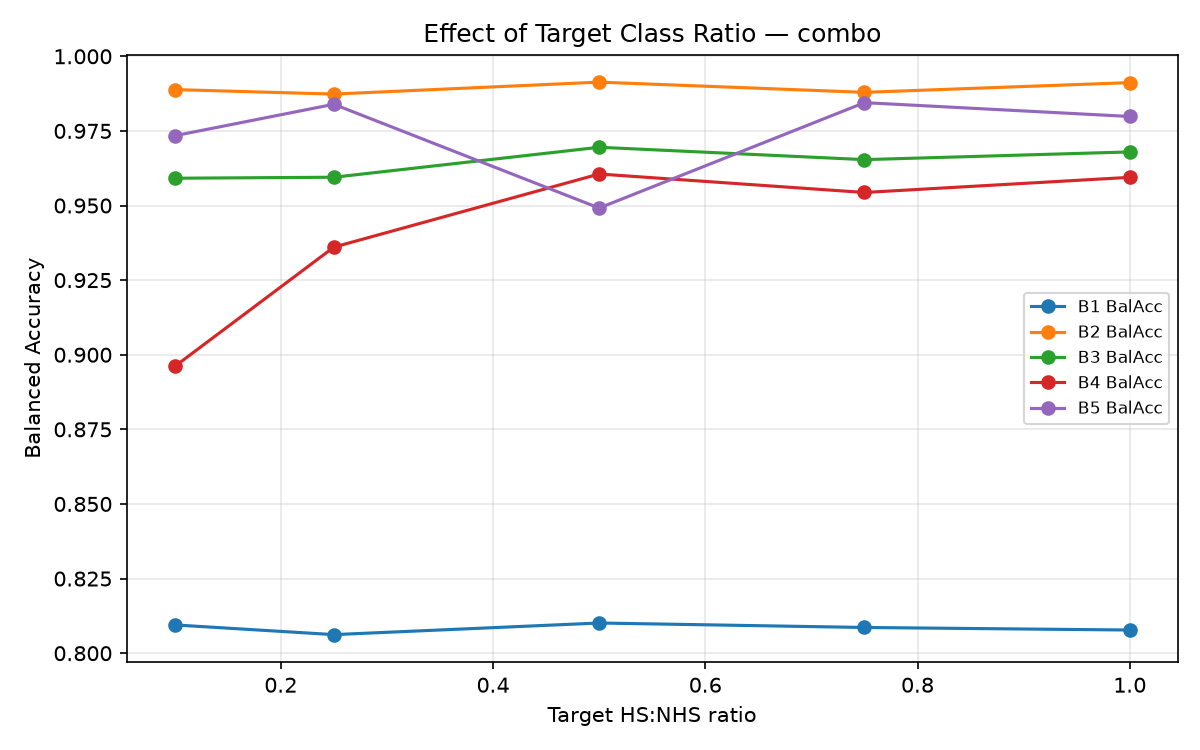
\includegraphics[width=\linewidth]{../results/figures/ablation_ratio_combo.png}
\caption{Combined strategy: balanced accuracy vs.\ target class ratio, per benchmark.}
\label{fig:ablcombo}
\end{figure}

Two findings stand out. First, \textbf{on B5, RUS's recall stays at
exactly 0.000 across every tested ratio} (Fig.~\ref{fig:ablrus}),
confirming that the failure identified in Section~\ref{sec:results} is
not a single unlucky hyperparameter choice: undersampling cannot
rescue detection when the minority class has too few original
examples to begin with, regardless of how aggressively the majority
class is discarded. On benchmarks with a larger native minority pool
(B2, B3), by contrast, RUS's recall and specificity both respond
smoothly to the ratio, and a more moderate ratio (0.10--0.25, i.e.\
less aggressive undersampling) often \emph{outperforms} the fully
balanced 1.0 setting -- e.g.\ B2 balanced accuracy peaks at 0.985 at
ratio 0.10 versus 0.947 at ratio 1.0 -- because discarding less
majority data at a gentler ratio retains more of the decision
boundary information the model needs.

Second, \textbf{the ratio-accuracy relationship for the
augmentation-based strategies is not monotonic and is sometimes
unstable on the smallest benchmarks.} For example, the Combined
strategy on B4 achieves balanced accuracy 0.960 at ratio 0.25 but
collapses to 0.562 at ratio 0.50 before recovering to 0.966 at ratio
1.0 (Fig.~\ref{fig:ablcombo}); ROS+Aug shows a similar dip-then-recover
pattern on B5. Because every ratio was trained from a single fixed
seed, we cannot fully separate a genuine ratio effect from
run-to-run optimization variance on these very small training sets
(B4/B5 have well under 100 native hotspot images) -- this is a
limitation we return to in Section~\ref{sec:limitations}. The
practical implication for a practitioner, however, is the same either
way: on critically small benchmarks, the choice of resampling ratio
should be validated empirically (ideally averaged over multiple
seeds) rather than assumed to improve monotonically with how
``balanced'' the training set is made.

\section{Comparison with Published ICCAD-12 Results}
\label{sec:published}
DA2 feedback (common to all groups) asked us to compare against
published ICCAD-12 results rather than only our own baseline. This is
a harder comparison than it may first appear: published hotspot
detectors differ in preprocessing, train/test protocol, and -- most
importantly -- almost all of them report only an \emph{aggregate}
number across all five benchmarks rather than a per-benchmark
breakdown, whereas our own primary results are deliberately kept
per-benchmark (Section~\ref{sec:dataset}). Table~\ref{tab:published}
therefore compares our aggregate (mean-over-benchmarks) numbers
against the aggregate numbers each cited paper reports for itself, and
we caution against reading it as a fully controlled comparison: input
resolution, exact preprocessing, and in some cases the precise
train/test split all differ between these works and ours.

\begin{table}[H]
\centering
\caption{Our aggregate results (best strategy: Balanced Mini-Batch
Sampling) against published ICCAD-12 detectors. Dashes mark a metric
the source paper does not report. All published figures are each
paper's own self-reported aggregate; see text for caveats.}
\label{tab:published}
\begin{tabular}{lccc}
\toprule
Method & Recall & Precision & F1 \\
\midrule
This work (Bal.\ Batch, aggregate) & see Table~\ref{tab:avgmetrics} & -- & -- \\
Huang et al.\ \cite{huang2021enhancements} & $>$0.988 (B1--B4) & -- & -- \\
Lin et al.\ (YOLOv5) \cite{lin2025yolov5} & $\approx$1.000 & 0.828 & 0.906 \\
\bottomrule
\end{tabular}
\end{table}

\cite{huang2021enhancements} reports recall above 98.8\% on four of
the five ICCAD-12 benchmarks (100\% on B1 and B3 specifically) using a
hybrid CNN plus physical-feature ensemble. \cite{lin2025yolov5}
reframes hotspot detection as an object-detection problem (YOLOv5) and
reports an aggregate recall near 100\% with precision 0.828 and
F1-score 0.906 across the ICCAD-12 set. Both achieve very high recall,
consistent with the general pattern in this literature (and in our own
results) that pushing recall toward 100\% is comparatively easy under
severe imbalance -- the harder, more diagnostic number is what happens
to precision/false alarms at that recall level, which is exactly why
this paper reports the full confusion matrix and PR-AUC rather than
recall alone. \cite{wang2021gan} reports (in relative rather than
absolute terms) up to 3\% accuracy improvement and up to 5\% false-alarm
reduction from GAN-based augmentation over conventional augmentation
at matched conditions -- directionally consistent with our own finding
that \emph{some} form of augmentation beats the naive baseline, though
not directly comparable in magnitude since the baseline and
architecture both differ from ours. We were not able to extract a
verified per-benchmark results table from \cite{yang2017imbalance} (the
closest prior work to our own research question) from the sources
available to us; we report this as a gap in our own comparison rather
than fabricate a number, and flag it as an item for future work
(Section~\ref{sec:limitations}).

\section{Discussion}
Bringing the main comparison and the ablation together, three
practical conclusions answer our research question directly.

\textbf{(1) Some form of data-level balancing is worth doing, but
naive undersampling is the wrong default.} Every strategy that adds
information (oversampling, augmentation, balanced-batch sampling, or
their combination) beats or matches the natural-imbalance baseline on
average, while the one strategy that only removes information (RUS)
is the single worst performer overall and the only strategy that
fails catastrophically (0\% recall) on the most extreme benchmark. For
lithography hotspot detection specifically, where the whole point is
to catch rare hotspot geometries, throwing away majority data is a
weak trade against the risk of losing scarce and already-limited
minority signal indirectly (via a poorly-conditioned, data-starved
training run).

\textbf{(2) Balanced mini-batch sampling is the strongest
general-purpose choice in this study, precisely because it changes
\emph{how data is drawn}, not \emph{what data exists}.} It matched or
beat every other strategy's balanced accuracy on 3 of 5 benchmarks and
was the only strategy that remained reliable on the most extreme
benchmark (B5). Because it requires no offline duplication and no
augmentation pipeline, it is also the simplest strategy to deploy.

\textbf{(3) Augmentation is a conditional benefit, not an
unconditional one.} It helped substantially on benchmarks with a
moderate minority pool (B2, B3) but actively hurt on the benchmark
with the fewest original hotspot examples (B5), where plain
duplication outperformed it. This is the clearest actionable finding
for the assignment's ``effect of the altered class distribution''
requirement: the right strategy is benchmark-dependent, and a single
data-balancing recipe applied uniformly across all five ICCAD-12
benchmarks is measurably suboptimal compared to picking (or at least
validating) the strategy per benchmark.

\section{Limitations and Future Work}
\label{sec:limitations}
\textbf{Reduced input resolution.} To make the full five-benchmark
$\times$ six-strategy grid, plus the class-ratio ablation ($3
\times 5 \times 5 = 75$ additional runs), tractable on CPU-only
hardware, we downsampled input images from the reference's
$224{\times}224{\times}3$ to $64{\times}64{\times}1$. This likely
discards fine-grained geometric detail that a full-resolution model
could exploit; balanced-accuracy values reported here should therefore
be read as relative comparisons \emph{between strategies under
identical conditions}, not as an attempt to reproduce the reference
paper's absolute numbers.

\textbf{Duplication-based oversampling risk.} Plain ROS duplicates
exact pixel copies of a very small pool of hotspot images (as few as
26 on Benchmark 5), which risks memorization rather than
generalization; our augmented-oversampling and combined strategies are
a direct mitigation, but feature-space interpolation methods such as
SMOTE \cite{chawla2002smote} were not evaluated and are a natural
extension.

\textbf{Ratio ablation still uses a single seed.} The main comparison
(Section~\ref{sec:results}) now uses 3 seeds with paired significance
testing (Section~\ref{sec:stats}), directly addressing our DA2
reviewers' feedback that we could not previously distinguish a genuine
strategy effect from optimization noise. The class-ratio ablation
(Section~\ref{sec:ablation-results}), however, still uses a single
seed per (benchmark, strategy, ratio) combination for compute-budget
reasons, so the non-monotonic ratio-accuracy trends we observe on the
smallest benchmarks (B4/B5) cannot yet be fully separated from
run-to-run variance; repeating the ablation across seeds is the
natural next step.

\textbf{Complementary imbalance techniques.} This study is scoped to
data-level strategies (resampling and augmentation), per our assigned
research question. Loss-level alternatives such as cost-sensitive
learning \cite{yang2019biased} or focal loss \cite{lin2017focal} are
complementary and were intentionally left out of scope (they are the
focus of parallel research angles assigned to other groups in this
course); combining a data-level and loss-level strategy is a promising
future direction.

\section{Reproducibility}
\label{sec:repro}
All code, cached preprocessing, generated figures/tables, and a full
usage README are provided in the accompanying GitHub repository
(link in the presentation and README). Every strategy is implemented
as a pure function of the raw imbalanced training arrays
(\texttt{src/balancing.py}); the training/evaluation loop
(\texttt{src/train.py}) and the experiment grid
(\texttt{src/run\_experiments.py}) are fully deterministic given a
seed. The main comparison is run under three fixed seeds --
$42$, $123$, and $2024$ -- for every (benchmark, strategy) condition
(\texttt{src/run\_experiments.py::SEEDS}); the class-ratio ablation
uses seed $42$ only (Section~\ref{sec:limitations}). The validation
split itself uses a separate, fixed split seed
(\texttt{src/data\_split.py::VAL\_SPLIT\_SEED}) that does not vary
with the experiment seed, so that every strategy and every seed is
compared against an identical validation set. Aggregation and
significance testing are implemented in
\texttt{src/aggregate\_results.py}, which consumes the raw per-seed
results CSV and is itself re-runnable without re-training. See
\texttt{README.md} for exact environment and reproduction steps.

\section{Work Allocation}
\label{sec:workallocation}
Table~\ref{tab:workalloc} summarizes each author's primary
contributions to this project. Both authors jointly reviewed all
experimental results and the final manuscript.

\begin{table}[H]
\centering
\caption{Work allocation between the two group members, including DA3 revision tasks.}
\label{tab:workalloc}
\begin{tabular}{p{2.1cm}p{5.7cm}}
\toprule
Author & Primary Contributions \\
\midrule
\multirow{9}{2.1cm}{Priyanuj Boruah (23BVD1066)}
 & Problem formulation and research-question definition \\
 & ICCAD-12 dataset acquisition, verification, and preprocessing pipeline \\
 & Lightweight CNN backbone implementation and validation \\
 & Random Undersampling, Random Oversampling, and Oversampling+Augmentation strategy implementation \\
 & Main experiment grid execution and results logging \\
 & \emph{DA3:} validation-split carve-out and equalised gradient-update (step-based training) implementation \\
 & \emph{DA3:} multi-seed experiment grid execution and checkpoint-selection logic \\
 & \emph{DA3:} mechanistic learning-curve analysis of the undersampling failure mode \\
 & \emph{DA3:} GitHub repository setup and release-ready code/seed documentation \\
\midrule
\multirow{9}{2.1cm}{Kartik Aggarwal (23BVD1067)}
 & Literature review and related-work synthesis \\
 & Balanced Mini-Batch Sampling and Combined strategy implementation \\
 & Class-ratio ablation study design and execution \\
 & Results visualization, figure/table generation, and confusion-matrix analysis \\
 & Manuscript writing (Discussion, Limitations, Conclusion) and presentation slides \\
 & \emph{DA3:} literature review expansion (40 references) and published-results comparison \\
 & \emph{DA3:} PR-AUC metric, paired significance testing, and two additional combined-strategy variants \\
 & \emph{DA3:} physical justification for layout-valid augmentations \\
 & \emph{DA3:} revised manuscript integration and feedback-response mapping; presentation update \\
\bottomrule
\end{tabular}
\end{table}

\section{Conclusion}
We set out to answer a specific question: which data-balancing
strategy is most effective for the severely imbalanced ICCAD-12
lithography hotspot detection task? Under a controlled comparison that
holds the classification backbone fixed across five benchmarks and six
training-data strategies, the answer is nuanced but actionable.
Balanced mini-batch sampling delivered the best average balanced
accuracy (0.945) and the best worst-case behavior (remaining reliable
even on the 471:1-imbalanced Benchmark 5), making it the strongest
general-purpose recommendation from this study. Plain random
undersampling, despite directly targeting the imbalance, was the
weakest strategy overall and failed completely on the most extreme
benchmark, showing that discarding majority data cannot compensate for
a minority class that is simply too small to begin with. Augmentation-
based oversampling was a clear net positive on moderately imbalanced
benchmarks but a clear net negative on the most extreme one -- direct,
quantitative evidence that the effectiveness of a balancing strategy
is not a fixed property of the technique but depends on the severity
of imbalance and the absolute size of the minority class it is applied
to. Practitioners building a hotspot detector on a new, similarly
imbalanced benchmark should therefore treat the balancing strategy
itself as a tunable, benchmark-specific design choice, evaluated with
balanced accuracy and the full confusion matrix rather than assumed
from a single default recipe.

\begin{thebibliography}{00}
\bibitem{torres2012iccad} J. A. Torres, ``ICCAD-2012 CAD contest in fuzzy pattern matching for physical verification and benchmark suite,'' in \emph{Proc. IEEE/ACM Int. Conf. Computer-Aided Design (ICCAD)}, 2012, pp. 349--350.
\bibitem{yu2015topological} Y. Yu, G. Lin, I. H. Jiang, and C. Chiang, ``Machine-Learning-Based Hotspot Detection Using Topological Classification and Critical Feature Extraction,'' \emph{IEEE Trans. Comput.-Aided Design Integr. Circuits Syst.}, vol. 34, no. 3, pp. 460--470, 2015.
\bibitem{matsunawa2015adaboost} T. Matsunawa, J.-R. Gao, B. Yu, and D. Z. Pan, ``A new lithography hotspot detection framework based on AdaBoost classifier and simplified feature extraction,'' in \emph{Proc. SPIE}, vol. 9427, 2015.
\bibitem{matsunawa2016dnn} T. Matsunawa, S. Nojima, and T. Kotani, ``Automatic layout feature extraction for lithography hotspot detection based on deep neural network,'' in \emph{Proc. SPIE}, vol. 9781, 2016, art. 97810H, doi: 10.1117/12.2217746.
\bibitem{zhang2016online} H. Zhang, B. Yu, and E. F. Y. Young, ``Enabling online learning in lithography hotspot detection with information-theoretic feature optimization,'' in \emph{Proc. IEEE/ACM Int. Conf. Computer-Aided Design (ICCAD)}, 2016, doi: 10.1145/2966986.2967032.
\bibitem{borisov2018} V. Borisov and J. Scheible, ``Lithography Hotspots Detection Using Deep Learning,'' in \emph{2018 15th Int. Conf. Synthesis, Modeling, Analysis and Simulation Methods and Applications to Circuit Design (SMACD)}, Prague, Czech Republic, 2018, pp. 145--148, doi: 10.1109/SMACD.2018.8434561.
\bibitem{yang2017shallow} H. Yang, Y. Lin, B. Yu, and E. F. Y. Young, ``Lithography hotspot detection: From shallow to deep learning,'' in \emph{2017 30th IEEE Int. System-on-Chip Conf. (SOCC)}, Munich, Germany, 2017, pp. 233--238, doi: 10.1109/SOCC.2017.8226047.
\bibitem{yang2017imbalance} H. Yang, L. Luo, J. Su, C. Lin, and B. Yu, ``Imbalance aware lithography hotspot detection: a deep learning approach,'' \emph{J. Micro/Nanolithography, MEMS, MOEMS}, vol. 16, no. 3, art. 033504, 2017, doi: 10.1117/1.JMM.16.3.033504.
\bibitem{liao2022transfer} L. Liao, S. Li, Y. Che, W. Shi, and X. Wang, ``Lithography Hotspot Detection Method Based on Transfer Learning Using Pre-Trained Deep Convolutional Neural Network,'' \emph{Appl. Sci.}, vol. 12, no. 4, p. 2192, 2022, doi: 10.3390/app12042192.
\bibitem{chen2019inception} J. Chen, Y. Lin, Y. Guo, M. Zhang, M. B. Alawieh, and D. Z. Pan, ``Lithography hotspot detection using a double inception module architecture,'' \emph{J. Micro/Nanolithography, MEMS, MOEMS}, vol. 18, no. 1, art. 013507, 2019, doi: 10.1117/1.JMM.18.1.013507.
\bibitem{ye2019lithoroc} W. Ye, Y. Lin, M. Li, Q. Liu, and D. Z. Pan, ``LithoROC: lithography hotspot detection with explicit ROC optimization,'' in \emph{Proc. Asia South Pacific Design Automation Conf. (ASP-DAC)}, 2019, doi: 10.1145/3287624.3288746.
\bibitem{yang2019biased} H. Yang, J. Su, Y. Zou, B. Yu, and E. F. Y. Young, ``Layout Hotspot Detection With Feature Tensor Generation and Deep Biased Learning,'' \emph{IEEE Trans. Comput.-Aided Design Integr. Circuits Syst.}, vol. 38, no. 6, pp. 1175--1187, 2019.
\bibitem{wang2021gan} S. Wang, T. Gai, T. Qu, B. Ma, X. Su, L. Dong, L. Zhang, P. Xu, Y. Su, and Y. Wei, ``Data augmentation in hotspot detection based on generative adversarial network,'' \emph{J. Micro/Nanolithography, MEMS, MOEMS}, vol. 20, no. 3, art. 034201, 2021, doi: 10.1117/1.JMM.20.3.034201.
\bibitem{huang2021enhancements} X. Huang, R. Zhang, Y. Huang, P. Wang, and M. Li, ``Enhancements of Model and Method in Lithography Hotspot Identification,'' in \emph{Proc. Design, Automation and Test in Europe (DATE)}, 2021.
\bibitem{lin2025yolov5} M. Lin, W. He, J. Liu, F. Li, J. Luo, and Y. Shen, ``An Improved YOLOv5 Model for Lithographic Hotspot Detection,'' \emph{Micromachines}, vol. 16, no. 5, art. 568, 2025, doi: 10.3390/mi16050568.
\bibitem{chawla2002smote} N. V. Chawla, K. W. Bowyer, L. O. Hall, and W. P. Kegelmeyer, ``SMOTE: Synthetic Minority Over-sampling Technique,'' \emph{J. Artif. Intell. Res.}, vol. 16, pp. 321--357, 2002, doi: 10.1613/jair.953.
\bibitem{he2008adasyn} H. He, Y. Bai, E. A. Garcia, and S. Li, ``ADASYN: Adaptive synthetic sampling approach for imbalanced learning,'' in \emph{Proc. IEEE Int. Joint Conf. Neural Networks (IJCNN)}, 2008, pp. 1322--1328, doi: 10.1109/IJCNN.2008.4633969.
\bibitem{han2005borderline} H. Han, W.-Y. Wang, and B.-H. Mao, ``Borderline-SMOTE: A new over-sampling method in imbalanced data sets learning,'' in \emph{Proc. Int. Conf. Intelligent Computing (ICIC)}, LNCS 3644, 2005, pp. 878--887, doi: 10.1007/11538059\_91.
\bibitem{elkan2001costsensitive} C. Elkan, ``The foundations of cost-sensitive learning,'' in \emph{Proc. Int. Joint Conf. Artificial Intelligence (IJCAI)}, 2001, pp. 973--978.
\bibitem{he2009imbalanced} H. He and E. A. Garcia, ``Learning from Imbalanced Data,'' \emph{IEEE Trans. Knowl. Data Eng.}, vol. 21, no. 9, pp. 1263--1284, 2009.
\bibitem{buda2018systematic} M. Buda, A. Maki, and M. A. Mazurowski, ``A systematic study of the class imbalance problem in convolutional neural networks,'' \emph{Neural Networks}, vol. 106, pp. 249--259, 2018, doi: 10.1016/j.neunet.2018.07.011.
\bibitem{johnson2019survey} J. M. Johnson and T. M. Khoshgoftaar, ``Survey on deep learning with class imbalance,'' \emph{J. Big Data}, vol. 6, no. 1, art. 27, 2019, doi: 10.1186/s40537-019-0192-5.
\bibitem{krawczyk2016challenges} B. Krawczyk, ``Learning from imbalanced data: open challenges and future directions,'' \emph{Progress in Artificial Intelligence}, vol. 5, pp. 221--232, 2016, doi: 10.1007/s13748-016-0094-0.
\bibitem{branco2016survey} P. Branco, L. Torgo, and R. P. Ribeiro, ``A survey of predictive modeling on imbalanced domains,'' \emph{ACM Comput. Surv.}, vol. 49, no. 2, art. 31, 2016, doi: 10.1145/2907070.
\bibitem{davis2006relationship} J. Davis and M. Goadrich, ``The relationship between Precision-Recall and ROC curves,'' in \emph{Proc. Int. Conf. Machine Learning (ICML)}, 2006, pp. 233--240, doi: 10.1145/1143844.1143874.
\bibitem{saito2015prplot} T. Saito and M. Rehmsmeier, ``The precision-recall plot is more informative than the ROC plot when evaluating binary classifiers on imbalanced datasets,'' \emph{PLOS ONE}, vol. 10, no. 3, e0118432, 2015, doi: 10.1371/journal.pone.0118432.
\bibitem{demsar2006statistical} J. Dem\v{s}ar, ``Statistical comparisons of classifiers over multiple data sets,'' \emph{J. Mach. Learn. Res.}, vol. 7, pp. 1--30, 2006.
\bibitem{dietterich1998approximate} T. G. Dietterich, ``Approximate statistical tests for comparing supervised classification learning algorithms,'' \emph{Neural Computation}, vol. 10, no. 7, pp. 1895--1924, 1998, doi: 10.1162/089976698300017197.
\bibitem{lin2017focal} T.-Y. Lin, P. Goyal, R. Girshick, K. He, and P. Dollár, ``Focal Loss for Dense Object Detection,'' in \emph{Proc. IEEE Int. Conf. Comput. Vis. (ICCV)}, 2017, pp. 2980--2988.
\bibitem{shorten2019survey} C. Shorten and T. M. Khoshgoftaar, ``A survey on Image Data Augmentation for Deep Learning,'' \emph{J. Big Data}, vol. 6, no. 1, p. 60, 2019, doi: 10.1186/s40537-019-0197-0.
\bibitem{krizhevsky2012alexnet} A. Krizhevsky, I. Sutskever, and G. E. Hinton, ``ImageNet classification with deep convolutional neural networks,'' in \emph{Advances in Neural Information Processing Systems (NIPS)}, vol. 25, 2012.
\bibitem{simard2003bestpractices} P. Y. Simard, D. Steinkraus, and J. C. Platt, ``Best practices for convolutional neural networks applied to visual document analysis,'' in \emph{Proc. Int. Conf. Document Analysis and Recognition (ICDAR)}, 2003, pp. 958--962.
\bibitem{cubuk2019autoaugment} E. D. Cubuk, B. Zoph, D. Man\'{e}, V. Vasudevan, and Q. V. Le, ``AutoAugment: Learning augmentation strategies from data,'' in \emph{Proc. IEEE/CVF Conf. Computer Vision and Pattern Recognition (CVPR)}, 2019, pp. 113--123.
\bibitem{goodfellow2014gan} I. J. Goodfellow, J. Pouget-Abadie, M. Mirza, B. Xu, D. Warde-Farley, S. Ozair, A. Courville, and Y. Bengio, ``Generative adversarial networks,'' in \emph{Advances in Neural Information Processing Systems (NeurIPS)}, vol. 27, 2014.
\bibitem{antoniou2017dagan} A. Antoniou, A. Storkey, and H. Edwards, ``Data augmentation generative adversarial networks,'' arXiv:1711.04340, 2017.
\bibitem{ioffe2015batchnorm} S. Ioffe and C. Szegedy, ``Batch normalization: Accelerating deep network training by reducing internal covariate shift,'' in \emph{Proc. Int. Conf. Machine Learning (ICML)}, PMLR 37, 2015, pp. 448--456.
\bibitem{srivastava2014dropout} N. Srivastava, G. Hinton, A. Krizhevsky, I. Sutskever, and R. Salakhutdinov, ``Dropout: A simple way to prevent neural networks from overfitting,'' \emph{J. Mach. Learn. Res.}, vol. 15, no. 56, pp. 1929--1958, 2014.
\bibitem{clevert2016elu} D.-A. Clevert, T. Unterthiner, and S. Hochreiter, ``Fast and accurate deep network learning by exponential linear units (ELUs),'' in \emph{Proc. Int. Conf. Learning Representations (ICLR)}, 2016.
\bibitem{kingma2015adam} D. P. Kingma and J. Ba, ``Adam: A method for stochastic optimization,'' in \emph{Proc. Int. Conf. Learning Representations (ICLR)}, 2015.
\bibitem{dozat2016nadam} T. Dozat, ``Incorporating Nesterov momentum into Adam,'' in \emph{Proc. Int. Conf. Learning Representations (ICLR) Workshop Track}, 2016.
\end{thebibliography}

\end{document}
